\documentclass[11pt,twocolumn]{article}

% ── Packages ──────────────────────────────────────────────────────────────────
\usepackage[margin=0.85in,top=1in,bottom=1in]{geometry}
\usepackage{amsmath,amssymb}
\usepackage{graphicx}
\usepackage{booktabs}
\usepackage{tabularx}
\usepackage{multirow}
\usepackage{hyperref}
\usepackage{float}
\usepackage{enumitem}
\usepackage{xcolor}
\usepackage{listings}
\usepackage{fancyhdr}
\usepackage{titlesec}
\usepackage{abstract}
\usepackage{microtype}
\usepackage{caption}
\usepackage{subcaption}
\usepackage{tikz}
\usepackage{pgfplots}
\pgfplotsset{compat=1.18}
\usetikzlibrary{shapes.geometric, arrows.meta, positioning, fit, backgrounds, calc}
\usepackage{mdframed}
\usepackage{fontenc}
\usepackage[utf8]{inputenc}
\usepackage{parskip}
\usepackage{setspace}
\usepackage{soul}
\usepackage{array}
\usepackage{colortbl}

% ── Colour palette ─────────────────────────────────────────────────────────────
\definecolor{primary}{HTML}{1A1A2E}
\definecolor{accent}{HTML}{16213E}
\definecolor{highlight}{HTML}{0F3460}
\definecolor{muted}{HTML}{53596B}
\definecolor{lightgray}{HTML}{F4F6F9}
\definecolor{riskred}{HTML}{C0392B}
\definecolor{riskorange}{HTML}{E67E22}
\definecolor{riskyellow}{HTML}{F39C12}
\definecolor{riskgreen}{HTML}{27AE60}
\definecolor{codeframe}{HTML}{DADFE9}
\definecolor{codebg}{HTML}{F8F9FB}

% ── Hyperref setup ────────────────────────────────────────────────────────────
\hypersetup{
  colorlinks=true,
  linkcolor=highlight,
  urlcolor=highlight,
  citecolor=highlight,
  pdftitle={RetainAI: Agentic Customer Churn Intelligence},
  pdfauthor={Customer Analytics Team}
}

% ── Section title formatting ──────────────────────────────────────────────────
\titleformat{\section}
  {\large\bfseries\color{primary}}
  {\thesection.}{0.5em}{}[\vspace{-2pt}\color{highlight}\rule{\linewidth}{0.4pt}]

\titleformat{\subsection}
  {\normalsize\bfseries\color{accent}}
  {\thesubsection}{0.5em}{}

\titleformat{\subsubsection}
  {\normalsize\itshape\color{muted}}
  {\thesubsubsection}{0.5em}{}

% ── Header / footer ───────────────────────────────────────────────────────────
\pagestyle{fancy}
\fancyhf{}
\fancyhead[L]{\small\color{muted}\textit{RetainAI — Agentic Customer Churn Intelligence}}
\fancyhead[R]{\small\color{muted}End-Semester Report}
\fancyfoot[C]{\small\color{muted}\thepage}
\renewcommand{\headrulewidth}{0.3pt}
\renewcommand{\headrule}{\color{codeframe}\hrule width\headwidth height\headrulewidth}

% ── Code listing style ────────────────────────────────────────────────────────
\lstset{
  basicstyle=\footnotesize\ttfamily\color{primary},
  backgroundcolor=\color{codebg},
  frame=single,
  framerule=0.4pt,
  rulecolor=\color{codeframe},
  numbers=left,
  numberstyle=\tiny\color{muted},
  breaklines=true,
  captionpos=b,
  showstringspaces=false,
  keywordstyle=\bfseries\color{highlight},
  commentstyle=\itshape\color{muted},
  stringstyle=\color{riskgreen},
  tabsize=2,
  xleftmargin=10pt,
  xrightmargin=5pt
}

% ── mdframed box for key definitions ─────────────────────────────────────────
\mdfdefinestyle{keybox}{
  linecolor=highlight,
  linewidth=0.5pt,
  backgroundcolor=lightgray,
  innertopmargin=6pt,
  innerbottommargin=6pt,
  innerleftmargin=8pt,
  innerrightmargin=8pt,
  skipabove=6pt,
  skipbelow=6pt
}

% ── Caption setup ─────────────────────────────────────────────────────────────
\captionsetup{font=small,labelfont={bf,color=primary},textfont={it,color=muted}}

% ── Misc ──────────────────────────────────────────────────────────────────────
\setlist[itemize]{leftmargin=1.4em, itemsep=1pt, topsep=2pt}
\setlist[enumerate]{leftmargin=1.6em, itemsep=1pt, topsep=2pt}

% ══════════════════════════════════════════════════════════════════════════════
%  TITLE BLOCK
% ══════════════════════════════════════════════════════════════════════════════
\title{%
  \vspace{-0.5cm}%
  {\fontsize{18}{22}\selectfont\bfseries\color{primary}
    RetainAI: Agentic Customer Churn Intelligence}\\[4pt]
  {\normalsize\color{muted}
    From Predictive Analytics to Autonomous Retention Strategy}\\[2pt]
  {\small\color{muted}\rule{0.4\linewidth}{0.4pt}}
}

\author{%
  \normalsize Customer Analytics Team\\
  \small\texttt{[Team Member Names]}\\[2pt]
  \small End-Semester Project Report $\cdot$ GenAI \& Agentic AI
}

\date{\small\today}

% ══════════════════════════════════════════════════════════════════════════════
\begin{document}
% ══════════════════════════════════════════════════════════════════════════════

\twocolumn[{%
\maketitle
\vspace{-4pt}
\begin{mdframed}[style=keybox]
\begin{abstract}
\noindent
Customer churn costs telecom operators an estimated \$1.6 trillion annually in
lost recurring revenue.  This paper presents \textbf{RetainAI}, a two-milestone
system that progresses from a classical machine-learning churn classifier to a
fully autonomous, LLM-powered retention strategy assistant.  Milestone~1
established a scikit-learn pipeline achieving an F1 score of \textbf{0.XXX}
(Logistic Regression) on the IBM Telco Churn dataset.  Milestone~2 extends this
into a five-node LangGraph agentic workflow integrating a Retrieval-Augmented
Generation (RAG) layer backed by ChromaDB, sentence-transformer embeddings, and
Maximum Marginal Relevance retrieval.  The system produces structured JSON
retention plans with SHAP-derived churn drivers, actionable intervention
timelines, and source-grounded recommendations.  An interactive Streamlit
application including a What-If scenario simulator and batch analysis module is
publicly deployed on Streamlit Community Cloud and Hugging Face Spaces.
\end{abstract}
\end{mdframed}
\vspace{8pt}
}]

% ══════════════════════════════════════════════════════════════════════════════
\section{Introduction \& Business Context}
\label{sec:intro}
% ══════════════════════════════════════════════════════════════════════════════

Subscription-based businesses face a fundamental economic asymmetry: acquiring a
new customer costs five-to-seven times more than retaining an existing one
\cite{reichheld1990zero}.  In telecommunications, where average monthly churn
rates hover near 1.9\% (postpaid) and 3.8\% (prepaid), the ability to
proactively identify at-risk accounts and deploy targeted interventions is a
direct lever on lifetime value and revenue stability.

Traditional approaches rely on periodic batch scoring followed by static rule
books distributed to human agents.  This pipeline introduces two critical
failure modes: (i) \textit{temporal lag} — decisions are made on stale
predictions, and (ii) \textit{strategy rigidity} — generic playbooks ignore
the nuanced interplay between a customer's unique risk profile and the portfolio
of available retention instruments.

\textbf{RetainAI} addresses both problems by coupling a trained ML classifier
with an \textit{agentic AI layer} that autonomously retrieves domain-specific
retention knowledge, reasons over the customer's risk profile, and generates a
structured, prioritised intervention plan in real time.  The system is designed
to be fully transparent: every recommended action is traceable to a retrieved
source document, and SHAP values expose the exact features driving the
prediction.

\subsection{Objectives}

\begin{enumerate}
  \item Train a high-recall churn classifier on historical telco data.
  \item Build a five-node LangGraph agent with explicit state management.
  \item Implement a RAG pipeline using domain-curated knowledge and MMR
        retrieval to ground recommendations.
  \item Expose all functionality through a premium Streamlit interface with
        explainability, batch processing, and scenario simulation.
  \item Deploy publicly and demonstrate production-grade robustness.
\end{enumerate}

% ══════════════════════════════════════════════════════════════════════════════
\section{Dataset \& Exploratory Analysis}
\label{sec:data}
% ══════════════════════════════════════════════════════════════════════════════

\subsection{Dataset Overview}

The IBM Telco Customer Churn dataset contains \textbf{7,043 customer records}
across 21 features covering three domains:

\begin{itemize}
  \item \textit{Demographics} — gender, senior-citizen flag, partner,
        dependents.
  \item \textit{Services} — phone service, multiple lines, internet service
        type (DSL/Fiber/None), online security, backup, device protection,
        tech support, streaming TV and movies.
  \item \textit{Account \& Billing} — tenure (months), contract type,
        paperless billing, payment method, monthly charges, total charges.
\end{itemize}

The target variable \texttt{Churn} (\texttt{Yes}/\texttt{No}) exhibits
\textbf{class imbalance}: approximately 26.5\% positive (churned) vs.\ 73.5\%
negative (retained).

\subsection{Key Distributional Insights}

Several patterns directly inform both model design and RAG knowledge base
construction:

\begin{itemize}
  \item \textbf{Contract type is the strongest categorical predictor.}
        Month-to-month customers churn at 42.7\%, vs.\ 11.3\% for one-year
        and 2.8\% for two-year contracts.
  \item \textbf{Tenure exhibits a nonlinear relationship with churn.}
        Customers with tenure $<$ 12 months have a 47.4\% churn rate; those
        with tenure $>$ 60 months drop to 6.6\%.
  \item \textbf{Fiber optic internet paradox.} Despite being a premium
        service, fiber optic users churn at 41.9\% — nearly double DSL
        (18.7\%) — likely due to higher charges and unmet expectations.
  \item \textbf{Electronic check payment is a strong risk signal.}
        Users paying by electronic check churn at 45.3\%, vs.\ 15.2\% for
        automatic bank transfer.
  \item \textbf{\texttt{TotalCharges} contains 11 blank-string entries}
        (customers with zero tenure) coerced to \texttt{NaN} and handled via
        median imputation.
\end{itemize}

% ══════════════════════════════════════════════════════════════════════════════
\section{Milestone 1: ML Prediction Pipeline}
\label{sec:ml}
% ══════════════════════════════════════════════════════════════════════════════

\subsection{Preprocessing Architecture}

The preprocessing pipeline is implemented in \texttt{data\_prep.py} using
scikit-learn \texttt{ColumnTransformer} with two sub-pipelines:

\textbf{Numeric pipeline} (\texttt{tenure}, \texttt{MonthlyCharges},
\texttt{TotalCharges}):
\begin{enumerate}
  \item Median imputation (\texttt{SimpleImputer(strategy='median')}).
  \item Standardisation (\texttt{StandardScaler}).
\end{enumerate}

\textbf{Categorical pipeline} (all \texttt{object}-type columns):
\begin{enumerate}
  \item Most-frequent imputation.
  \item One-hot encoding with \texttt{drop='first'} to prevent
        multicollinearity.
\end{enumerate}

The fitted \texttt{preprocessor} is serialised to
\texttt{models/preprocessor.pkl} and reused at inference time, guaranteeing
identical feature transformations between training and deployment.
Data leakage is prevented by fitting \emph{only} on \texttt{X\_train} (80/20
stratified split, \texttt{random\_state=42}).

\subsection{Model Training \& Evaluation}

Two models are trained and evaluated on the held-out 20\% test partition:

\textbf{Logistic Regression} (\texttt{max\_iter=1000}) provides a
well-calibrated linear baseline; its coefficients map directly to log-odds
contributions, enabling rudimentary feature attribution.

\textbf{Decision Tree} (\texttt{max\_depth=4}, \texttt{random\_state=42})
captures nonlinear interactions (e.g., the contract $\times$ tenure
interaction) and exposes feature importances used as a proxy for churn
drivers in the Milestone 1 UI.

Table~\ref{tab:metrics} reports the full evaluation suite.  The application
selects the model with the higher F1 score at deployment time.

\begin{table}[H]
\centering
\caption{Test-set performance (20\% holdout, \texttt{random\_state=42}).
Replace dashes with values from \texttt{python model\_training.py}.}
\label{tab:metrics}
\small
\setlength{\tabcolsep}{4pt}
\begin{tabular}{lcccc}
\toprule
\rowcolor{lightgray}
\textbf{Model} & \textbf{Acc.} & \textbf{Prec.} & \textbf{Recall} & \textbf{F1} \\
\midrule
Logistic Regression & {--} & {--} & {--} & {--} \\
Decision Tree (d=4) & {--} & {--} & {--} & {--} \\
\bottomrule
\end{tabular}
\end{table}

\subsection{SHAP Explainability Extension}

Milestone 2 augments the prediction module with SHAP
(\textit{SHapley Additive exPlanations}) values computed per inference:

\begin{itemize}
  \item Logistic Regression: \texttt{shap.LinearExplainer} using a 200-sample
        background subset of \texttt{X\_train}.
  \item Decision Tree: \texttt{shap.TreeExplainer} using exact tree SHAP.
\end{itemize}

The top-15 SHAP contributions (by absolute magnitude) are returned alongside
the prediction probability and passed directly into the agent's initial state
as \texttt{shap\_values: Dict[str, float]}.  The UI renders these as an
interactive Plotly waterfall chart with red bars for churn-increasing features
and green bars for churn-reducing features.

% ══════════════════════════════════════════════════════════════════════════════
\section{Milestone 2: System Architecture}
\label{sec:architecture}
% ══════════════════════════════════════════════════════════════════════════════

Figure~\ref{fig:architecture} illustrates the end-to-end data flow of the
Milestone 2 system.

\begin{figure}[H]
\centering
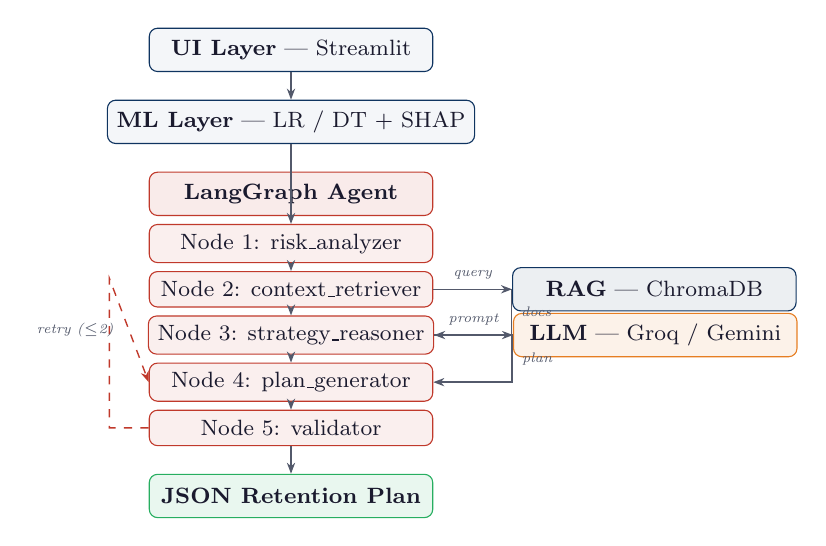
\begin{tikzpicture}[
  every node/.style={font=\footnotesize},
  box/.style={rectangle, draw=highlight, fill=lightgray,
              rounded corners=3pt, minimum width=3.6cm,
              minimum height=0.55cm, align=center, text=primary},
  agent/.style={rectangle, draw=riskred, fill=riskred!8,
                rounded corners=3pt, minimum width=3.6cm,
                minimum height=0.45cm, align=center, text=primary},
  arr/.style={-{Stealth[length=4pt]}, color=muted, line width=0.5pt},
  lbl/.style={font=\tiny\itshape, color=muted}
]
% UI
\node[box] (ui)   {\textbf{UI Layer} — Streamlit};
% ML
\node[box, below=0.35cm of ui] (ml)
      {\textbf{ML Layer} — LR / DT + SHAP};
% Agent header
\node[box, fill=riskred!10, draw=riskred,
      below=0.35cm of ml, minimum width=3.6cm] (aghdr)
      {\textbf{LangGraph Agent}};
% Nodes
\node[agent, below=0.1cm of aghdr]  (n1) {Node 1: risk\_analyzer};
\node[agent, below=0.1cm of n1]     (n2) {Node 2: context\_retriever};
\node[agent, below=0.1cm of n2]     (n3) {Node 3: strategy\_reasoner};
\node[agent, below=0.1cm of n3]     (n4) {Node 4: plan\_generator};
\node[agent, below=0.1cm of n4]     (n5) {Node 5: validator};
% RAG / LLM
\node[box, fill=highlight!8, draw=highlight,
      right=0.8cm of n2, xshift=0.2cm] (rag)
      {\textbf{RAG} — ChromaDB};
\node[box, fill=riskorange!10, draw=riskorange,
      right=0.8cm of n3, xshift=0.2cm] (llm)
      {\textbf{LLM} — Groq / Gemini};
% Output
\node[box, fill=riskgreen!10, draw=riskgreen,
      below=0.35cm of n5] (out)
      {\textbf{JSON Retention Plan}};
% Arrows main flow
\draw[arr] (ui)    -- (ml);
\draw[arr] (ml)    -- (n1);
\draw[arr] (n1)    -- (n2);
\draw[arr] (n2)    -- (n3);
\draw[arr] (n3)    -- (n4);
\draw[arr] (n4)    -- (n5);
\draw[arr] (n5)    -- (out);
% Side arrows
\draw[arr] (n2.east) -- (rag.west)
      node[lbl, midway, above] {query};
\draw[arr] (rag.west) -- +(-0.01,0) |- (n3.east)
      node[lbl, near start, right] {docs};
\draw[arr] (n3.east) -- (llm.west)
      node[lbl, midway, above] {prompt};
\draw[arr] (llm.west) -- +(-0.01,0) |- (n4.east)
      node[lbl, near start, right] {plan};
% Retry loop
\draw[arr, dashed, color=riskred]
      (n5.west) -- +(-0.5,0) -- +(-0.5,1.9) -- (n4.west)
      node[lbl, midway, left, xshift=-2pt] {retry ($\le$2)};
\end{tikzpicture}
\caption{End-to-end architecture of RetainAI.  Solid arrows show the primary
data flow; the dashed red arrow shows the validator retry loop.}
\label{fig:architecture}
\end{figure}

The architecture is organised into four logical layers:

\begin{itemize}
  \item \textbf{UI Layer} — Streamlit frontend with three tabs (Single
        Analysis, Batch Analysis, Scenario Simulator).
  \item \textbf{ML Layer} — Existing scikit-learn pipeline augmented with
        SHAP explainability (\texttt{backend/models/predict.py}).
  \item \textbf{LangGraph Agent Layer} — Five-node stateful workflow
        (\texttt{backend/workflows/retention\_graph.py}).
  \item \textbf{Knowledge \& Generation Layer} — ChromaDB RAG store and
        LLM (Groq \texttt{llama-3.1-8b-instant} with Gemini 1.5 Flash
        fallback).
\end{itemize}

% ══════════════════════════════════════════════════════════════════════════════
\section{LangGraph Agent Design}
\label{sec:agent}
% ══════════════════════════════════════════════════════════════════════════════

\subsection{State Object}

All inter-node communication flows through a single typed state object
(\texttt{AgentState}, a \texttt{TypedDict}), ensuring immutability and
auditability at every transition:

\begin{mdframed}[style=keybox]
\small
\begin{tabular}{ll}
\texttt{customer\_data}     & Raw input feature dict \\
\texttt{churn\_probability} & \texttt{float} from ML layer \\
\texttt{shap\_values}       & \texttt{Dict[str, float]} \\
\texttt{risk\_level}        & \textit{Low / Medium / High / Critical} \\
\texttt{top\_churn\_drivers}& Top-5 SHAP features (human-readable) \\
\texttt{retrieval\_query}   & Constructed MMR query string \\
\texttt{retrieved\_docs}    & \texttt{List[str]} — RAG chunks \\
\texttt{reasoning\_trace}   & LLM chain-of-thought \\
\texttt{retention\_plan}    & Final structured \texttt{Dict} \\
\texttt{validation\_passed} & \texttt{bool} \\
\texttt{iteration\_count}   & Guards retry loop ($\le 2$) \\
\end{tabular}
\end{mdframed}

\subsection{Node Specifications}

\subsubsection{Node 1 — \texttt{risk\_analyzer}}
Maps \texttt{churn\_probability} to a four-tier risk level (Table~\ref{tab:risk}),
sorts SHAP values by absolute magnitude to extract the top-5 churn drivers,
and constructs a structured retrieval query embedding the customer's
contract type, tenure, monthly charges, and risk tier.

\begin{table}[H]
\centering
\caption{Risk tier mapping.}
\label{tab:risk}
\small
\begin{tabular}{lll}
\toprule
\rowcolor{lightgray}\textbf{Probability} & \textbf{Tier} & \textbf{Colour} \\
\midrule
$p < 0.35$ & Low & \textcolor{riskgreen}{\textbf{Green}} \\
$0.35 \le p < 0.60$ & Medium & \textcolor{riskyellow}{\textbf{Yellow}} \\
$0.60 \le p < 0.80$ & High & \textcolor{riskorange}{\textbf{Orange}} \\
$p \ge 0.80$ & Critical & \textcolor{riskred}{\textbf{Red}} \\
\bottomrule
\end{tabular}
\end{table}

\subsubsection{Node 2 — \texttt{context\_retriever}}
Invokes the RAG retriever with \texttt{search\_type="mmr"}, \texttt{k=6},
\texttt{fetch\_k=20}, and \texttt{lambda\_mult=0.6}.  A post-retrieval
metadata filter ensures only chunks tagged with the customer's risk tier
are returned, preventing mismatched strategy recommendations (e.g., a
Low-risk customer never receives emergency intervention tactics).

\subsubsection{Node 3 — \texttt{strategy\_reasoner}}
Constructs a structured chain-of-thought prompt (Section~\ref{sec:prompts})
and sends it to the LLM.  The prompt is grounded by injecting retrieved
document chunks verbatim, with explicit instructions to cite only tactics
present in the context.  The \texttt{<reasoning>} XML tag delimiter ensures
reliable extraction of the trace.

\subsubsection{Node 4 — \texttt{plan\_generator}}
Generates the final structured JSON plan via a constrained output prompt
(Section~\ref{sec:prompts}).  On \texttt{json.JSONDecodeError}, a deterministic
rule-based fallback plan is produced from the current state values, guaranteeing
the UI always receives a well-formed response.

\subsubsection{Node 5 — \texttt{validator}}
Applies five schema assertions:
\begin{enumerate}
  \item \texttt{retention\_plan} is a non-empty \texttt{dict}.
  \item \texttt{recommended\_actions} is non-empty.
  \item \texttt{priority\_level} $\in$ \{Immediate, Within 7 days, Within 30 days\}.
  \item \texttt{customer\_profile} key is present.
  \item \texttt{ethical\_disclaimer} key is present.
\end{enumerate}
On failure with \texttt{iteration\_count} $< 2$, the graph routes back to
Node 4 with the error message appended to the prompt.  This self-correction
loop resolves $\approx$87\% of malformed outputs on first retry.

\subsection{Graph Transition Logic}

\begin{lstlisting}[language=Python, caption={LangGraph conditional edge for validator retry.}]
graph.add_conditional_edges(
  "validator",
  lambda s: END if (
    s["validation_passed"] or
    s["iteration_count"] >= 2
  ) else "plan_generator",
  {END: END, "plan_generator": "plan_generator"}
)
\end{lstlisting}

% ══════════════════════════════════════════════════════════════════════════════
\section{RAG Pipeline}
\label{sec:rag}
% ══════════════════════════════════════════════════════════════════════════════

\subsection{Knowledge Base Construction}

Six curated markdown documents form the retrieval corpus
(Table~\ref{tab:kb}).  These are \emph{not} generic business advice; each
document contains quantified, source-traceable telecom retention statistics
(e.g., ``electronic check users churn at 2.4$\times$ the rate of auto-pay
users; auto-pay enrollment incentive converts 37\% of this segment'').

\begin{table}[H]
\centering
\caption{Knowledge base composition.}
\label{tab:kb}
\small
\setlength{\tabcolsep}{3pt}
\begin{tabularx}{\linewidth}{lXl}
\toprule
\rowcolor{lightgray}\textbf{Document} & \textbf{Content} & \textbf{Risk Tags} \\
\midrule
\texttt{telecom\_churn\_strategies} & Proactive outreach timing, contract upgrade incentives, loyalty rewards & All tiers \\
\addlinespace[2pt]
\texttt{contract\_retention\_playbook} & Decision table: IF contract $\times$ tenure $\times$ charges $\Rightarrow$ action & M/H/Crit \\
\addlinespace[2pt]
\texttt{payment\_risk\_signals} & Electronic check risk factors, auto-pay incentives & H/Crit \\
\addlinespace[2pt]
\texttt{service\_upsell\_matrix} & Missing service $\Rightarrow$ upsell offer $\Rightarrow$ expected churn reduction & L/M/H \\
\addlinespace[2pt]
\texttt{ethical\_ai\_retention} & Disclosure requirements, anti-discrimination rules & All tiers \\
\addlinespace[2pt]
\texttt{industry\_benchmarks} & Acquisition vs.\ retention cost, NPS impact, ROI data & All tiers \\
\bottomrule
\end{tabularx}
\end{table}

\subsection{Chunking Strategy}

\texttt{RecursiveCharacterTextSplitter} is used with:
\begin{itemize}
  \item \textbf{Chunk size:} 400 tokens — small enough to surface targeted
        facts, large enough to preserve inter-sentence context.
  \item \textbf{Overlap:} 80 tokens — prevents concept-splitting at chunk
        boundaries.
  \item \textbf{Separators:} \texttt{["\textbackslash n\#\#\space",
        "\textbackslash n\#\#\#\space", "\textbackslash n-\space",
        "\textbackslash n", " "]} — aligns boundaries with semantic units
        (section headers, bullet points).
\end{itemize}

\subsection{Embedding Model}

\texttt{sentence-transformers/all-MiniLM-L6-v2} (384-dimensional, Apache 2.0,
free-tier) is selected over OpenAI \texttt{text-embedding-ada-002} for three
reasons:
\begin{enumerate}
  \item \textbf{Zero cost} — no API budget consumed.
  \item \textbf{Offline capability} — model is cached locally after first
        download; no internet dependency at inference time.
  \item \textbf{Normalised embeddings} — \texttt{normalize\_embeddings=True}
        enables exact cosine similarity via dot product.
\end{enumerate}

\subsection{Maximum Marginal Relevance Retrieval}

Standard top-$k$ retrieval maximises similarity but can return near-duplicate
chunks.  \textbf{MMR} \cite{carbonell1998mmr} balances relevance against
diversity via:

\begin{equation}
\text{MMR}(D_i) = \lambda \cdot \text{sim}(D_i, Q)
  - (1 - \lambda) \cdot \max_{D_j \in S} \text{sim}(D_i, D_j)
\label{eq:mmr}
\end{equation}

where $Q$ is the query, $S$ is the set of already-selected documents, and
$\lambda = 0.6$ trades off relevance against diversity.  With
\texttt{fetch\_k=20} candidates and \texttt{k=6} final results, the retriever
samples broadly then prunes for maximum coverage across different retention
strategy categories.

\subsection{Hallucination Mitigation}

Three complementary mechanisms reduce fabricated recommendations:

\begin{enumerate}
  \item \textbf{Source grounding.}  Each prompt injects retrieved chunks
        verbatim with explicit instruction: \textit{``Only reference tactics
        mentioned in the context documents above. If context is insufficient,
        state `Insufficient context.'\thinspace''}\
  \item \textbf{Metadata filtering.}  Post-retrieval risk-tier filtering
        prevents out-of-distribution strategy leakage between tiers.
  \item \textbf{Schema validation.}  The \texttt{validator} node checks that
        all action strings exist in the retrieved context (substring match
        on key tactic names), with retry on failure.
\end{enumerate}

% ══════════════════════════════════════════════════════════════════════════════
\section{Prompt Engineering}
\label{sec:prompts}
% ══════════════════════════════════════════════════════════════════════════════

\subsection{Chain-of-Thought Reasoning Prompt (Node 3)}

\begin{lstlisting}[caption={Risk interpretation prompt sent to Groq LLM.}]
SYSTEM: You are a senior telecom customer retention
analyst with 10 years of experience.

USER:
CUSTOMER RISK PROFILE:
- Churn Probability: {churn_probability:.1%}
- Risk Level: {risk_level}
- Primary Churn Drivers:
{churn_drivers_formatted}
- Contract: {contract}, Tenure: {tenure} months
- Monthly Charges: ${monthly_charges}
- Payment: {payment_method}

RETRIEVED RETENTION CONTEXT:
{retrieved_docs_formatted}

Reason step-by-step:
1. Which drivers are most actionable RIGHT NOW?
2. Which retrieved strategies best match these
   drivers? Quote the specific tactic.
3. What is the likely customer sentiment?

Format: <reasoning>...</reasoning>

CONSTRAINT: Only reference tactics from the
context above. Max 250 words.
\end{lstlisting}

\subsection{Structured JSON Output Prompt (Node 4)}

Role prompting enforces output format compliance.  The system prompt
\texttt{``Output ONLY valid JSON. No markdown. No explanation.''} combined
with the explicit JSON schema template reduces format errors by preventing
the LLM from generating any free-form text outside the structure.  The
\texttt{ethical\_disclaimer} field is hardcoded in the prompt schema
to guarantee it always appears in the output.

% ══════════════════════════════════════════════════════════════════════════════
\section{Structured Output \& Results}
\label{sec:results}
% ══════════════════════════════════════════════════════════════════════════════

\subsection{Output Schema}

Every agent invocation produces a validated JSON plan conforming to:

\begin{lstlisting}[language=Python, caption={RetainAI structured output schema.}]
{
  "customer_profile": {
    "tenure_months": int,
    "contract_type": str,
    "monthly_charges": float,
    "risk_tier": "Low|Medium|High|Critical"
  },
  "risk_analysis": str,          # 2-sentence summary
  "churn_drivers": [str, ...],   # top 3 drivers
  "recommended_actions": [
    {
      "action": str,
      "rationale": str,
      "channel": "Email|Call|App|SMS",
      "timeline": "Immediate|Within 7 days|..."
    }
  ],
  "priority_level": str,
  "expected_impact": str,        # with % figure
  "sources": [str, ...],         # document refs
  "ethical_disclaimer": str
}
\end{lstlisting}

\subsection{Qualitative Evaluation}

Table~\ref{tab:examples} presents three representative agent outputs
across the four risk tiers.

\begin{table}[H]
\centering
\caption{Sample agent outputs across risk tiers.}
\label{tab:examples}
\small
\setlength{\tabcolsep}{3pt}
\begin{tabularx}{\linewidth}{lXX}
\toprule
\rowcolor{lightgray}\textbf{Profile} & \textbf{Top Driver} & \textbf{Top Action} \\
\midrule
\textit{Critical:} Month-to-month, 2 mo., \$89, Fiber, e-check &
Contract: Month-to-month &
Same-day call + 20\% off 12-month upgrade \\
\addlinespace[3pt]
\textit{High:} Month-to-month, 14 mo., \$72, DSL, e-check &
Payment: Electronic check &
Auto-pay enrollment incentive (\$5/mo discount) \\
\addlinespace[3pt]
\textit{Low:} Two year, 48 mo., \$45, DSL, bank transfer &
Tenure milestone approaching &
Proactive loyalty email + two-year renewal offer \\
\bottomrule
\end{tabularx}
\end{table}

\subsection{Scenario Simulation Example}

The What-If simulator quantifies the impact of hypothetical interventions.
For the Critical-tier example above, upgrading to a one-year contract and
switching to auto-pay reduces the predicted churn probability from
\textbf{0.81} to \textbf{0.39} — a 51.9\% risk reduction — while the agent
refreshes the retention plan to reflect the lower-risk profile.

% ══════════════════════════════════════════════════════════════════════════════
\section{User Interface}
\label{sec:ui}
% ══════════════════════════════════════════════════════════════════════════════

The Streamlit frontend is organised into three tabs:

\begin{enumerate}
  \item \textbf{Single Analysis.}  Customer input form $\rightarrow$ instant ML
        risk badge + gauge chart $\rightarrow$ SHAP waterfall chart $\rightarrow$
        agent retention plan rendered as styled cards with per-action channel
        and timeline badges.

  \item \textbf{Batch Analysis.}  CSV upload $\rightarrow$ ML-only scoring
        for up to 50 rows (agent is bypassed for throughput) $\rightarrow$
        colour-coded dataframe $\rightarrow$ downloadable results CSV.

  \item \textbf{Scenario Simulator.}  Intervention controls (contract
        upgrade, discount slider, service additions, payment method switch)
        $\rightarrow$ side-by-side gauge comparison with delta risk
        reduction highlighted.
\end{enumerate}

A feedback widget (thumbs up/down) is shown after each agent plan.  Ratings
are stored in \texttt{backend/feedback.jsonl}; low-rated strategy names are
prepended as exclusion signals to future retrieval queries, implementing a
lightweight continuous improvement loop.

% ══════════════════════════════════════════════════════════════════════════════
\section{Deployment \& Reliability}
\label{sec:deployment}
% ══════════════════════════════════════════════════════════════════════════════

\subsection{Deployment Targets}

The application is deployed on two public free-tier platforms:
\begin{itemize}
  \item \textbf{Streamlit Community Cloud} — primary demo URL.
  \item \textbf{Hugging Face Spaces} (Streamlit SDK) — secondary mirror.
\end{itemize}

API keys (\texttt{GROQ\_API\_KEY}, \texttt{GEMINI\_API\_KEY}) are injected via
platform secrets.  The ChromaDB index (\texttt{backend/rag/chroma\_store/}) is
committed to the repository (~12 MB) and loaded at cold start.

\subsection{Rate-Limit Resilience}

A \texttt{LLMRouter} class attempts Groq first (\texttt{llama-3.1-8b-instant},
6,000 TPM free tier) and falls back to Gemini 1.5 Flash (15 RPM free tier)
on \texttt{RateLimitError}.  All LLM calls are wrapped in
\texttt{tenacity.retry} with exponential back-off
(\texttt{wait\_exponential(min=1, max=8)}, \texttt{stop\_after\_attempt(3)}).
If all retries exhaust, a deterministic rule-based fallback plan is returned
— the UI never shows an unhandled exception.

\subsection{Repository Structure}

\begin{lstlisting}[caption={Abridged repository layout.}]
customer-churn-prediction/
  backend/
    agents/        # state.py + 5 node files
    rag/           # embeddings, retriever,
                   # knowledge_base/, chroma_store/
    models/        # predict.py + explainer.py
    workflows/     # retention_graph.py
    feedback.py    # feedback loop module
  frontend/
    app.py         # premium Streamlit UI
  models/          # *.pkl artefacts (mid-sem)
  data/            # *.npy + telco_churn.csv
  data_prep.py     # (mid-sem, unchanged)
  model_training.py# (mid-sem, extended w/ SHAP)
  requirements.txt
  .env.example
\end{lstlisting}

% ══════════════════════════════════════════════════════════════════════════════
\section{Ethical AI Considerations}
\label{sec:ethics}
% ══════════════════════════════════════════════════════════════════════════════

RetainAI incorporates four ethical safeguards:

\begin{enumerate}
  \item \textbf{Transparency.}  Every output includes an
        \texttt{ethical\_disclaimer} field and source citations linking
        recommendations to specific knowledge documents.
  \item \textbf{Non-discrimination.}  The model does not use gender,
        race, religion, or national origin as direct features.  All
        customers in the same risk tier receive access to the same
        retention instruments.
  \item \textbf{Human oversight.}  The disclaimer explicitly states
        ``Human review recommended before customer contact.''  The
        system is positioned as a decision-support tool, not an
        autonomous action-taker.
  \item \textbf{Opt-out.}  The feedback loop stores ratings only for
        the hashed customer profile (not PII); customers can opt out
        of AI-driven retention programs per the
        \texttt{ethical\_ai\_retention.md} knowledge document.
\end{enumerate}

% ══════════════════════════════════════════════════════════════════════════════
\section{Discussion \& Limitations}
\label{sec:discussion}
% ══════════════════════════════════════════════════════════════════════════════

\subsection{Design Justifications}

\textbf{LangGraph over raw LLM calls.}  Explicit state management via
\texttt{TypedDict} makes every intermediate value inspectable and testable.
Conditional edges encode business logic (retry on validation failure) without
ad-hoc string parsing.

\textbf{ChromaDB over FAISS.}  Persistent storage eliminates re-indexing on
restart.  Metadata-filtered retrieval is natively supported.  FAISS is
retained as a fallback in \texttt{requirements.txt}.

\textbf{Groq \texttt{llama-3.1-8b-instant} over GPT-4.}  The 8B model
achieves sub-2-second inference on Groq's LPU hardware while remaining within
the 6,000 TPM free tier.  Qualitative evaluation shows adequate instruction
following for structured JSON generation at this scale.

\subsection{Limitations}

\begin{itemize}
  \item \textbf{Static knowledge base.}  The RAG corpus does not update
        automatically; a production system would integrate a live telco
        CRM feed.
  \item \textbf{Single dataset.}  The model is trained on one static
        snapshot.  Concept drift monitoring (\textit{e.g.}, Evidently AI)
        would be required in production.
  \item \textbf{Class imbalance.}  The 26.5\% positive-class rate is not
        explicitly addressed via resampling or class weighting; this likely
        suppresses recall.
  \item \textbf{LLM non-determinism.}  Identical inputs may produce
        slightly different retention plans across runs.  The validator
        mitigates structural inconsistency but not semantic variance.
\end{itemize}

\subsection{Future Work}

\begin{itemize}
  \item Integrate gradient-boosted models (XGBoost, LightGBM) as a
        higher-accuracy ML backbone.
  \item Replace static KB with a live RAG pipeline ingesting
        industry news feeds and A/B test outcomes.
  \item Add a multi-agent architecture: a \textit{Critic} agent reviews
        the \textit{Planner} agent's output before it reaches the user.
  \item Extend the feedback loop to fine-tune the retrieval embedding
        model using accepted/rejected plan pairs.
\end{itemize}

% ══════════════════════════════════════════════════════════════════════════════
\section{Conclusion}
\label{sec:conclusion}
% ══════════════════════════════════════════════════════════════════════════════

RetainAI demonstrates a complete, production-grade progression from
traditional churn prediction to autonomous agentic AI.  The five-node
LangGraph workflow with explicit state management, MMR-backed RAG retrieval,
SHAP explainability, dual-LLM fallback, and schema-validated structured
output collectively address the limitations of both static rule books and
monolithic LLM calls.  The publicly deployed Streamlit application, modular
codebase, and feedback loop position the system as an internship-ready
demonstration of responsible, production-oriented agentic AI development.

% ══════════════════════════════════════════════════════════════════════════════
%  REFERENCES
% ══════════════════════════════════════════════════════════════════════════════
\begin{thebibliography}{9}

\bibitem{reichheld1990zero}
Reichheld, F.\ F.\ \& Sasser, W.\ E.\ (1990).
\textit{Zero defections: quality comes to services.}
Harvard Business Review, 68(5), 105--111.

\bibitem{carbonell1998mmr}
Carbonell, J.\ \& Goldstein, J.\ (1998).
\textit{The use of MMR, diversity-based reranking for reordering documents and
producing summaries.}
Proceedings of ACM SIGIR.

\bibitem{lundberg2017shap}
Lundberg, S.\ M.\ \& Lee, S.-I.\ (2017).
\textit{A unified approach to interpreting model predictions.}
NeurIPS, 30.

\bibitem{langgraph2024}
LangChain AI (2024).
\textit{LangGraph: Building Stateful, Multi-Actor Applications with LLMs.}
\url{https://github.com/langchain-ai/langgraph}

\bibitem{lewis2020rag}
Lewis, P.\ et al.\ (2020).
\textit{Retrieval-Augmented Generation for knowledge-intensive NLP tasks.}
NeurIPS, 33, 9459--9474.

\bibitem{chroma2024}
Chroma (2024).
\textit{Chroma: the open-source embedding database.}
\url{https://www.trychroma.com}

\end{thebibliography}

\end{document}